% SPDX-License-Identifier: CC-BY-4.0
%
% Copyright (c) 2023 Nelson Vieira
%
% @author Nelson Vieira <nelson0.vieira@gmail.com>
% @license CC-BY-4.0 <https://creativecommons.org/licenses/by/4.0/legalcode.txt>
\documentclass{scrreprt}
\usepackage{cite}
\usepackage{listings}
\usepackage{underscore}
\usepackage{graphicx}
% \usepackage[tableposition=below]{caption}
% \captionsetup[longtable]{skip=1em}
\usepackage{amsmath,amssymb,amsfonts}
\usepackage{algorithmic}
\usepackage[T1]{fontenc}
\usepackage[table]{xcolor}
\usepackage{adjustbox}
% \usepackage{array,longtable,ltxtable,filecontents}
\usepackage{float}
% \usepackage{showframe}
% \renewcommand*\ShowFrameColor{\color{red}}
\def\UrlBreaks{\do\/\do-}
\def\BibTeX{{\rm B\kern-.05em{\sc i\kern-.025em b}\kern-.08em
    T\kern-.1667em\lower.7ex\hbox{E}\kern-.125emX}}
\usepackage[bookmarks=true]{hyperref}
\usepackage[utf8]{inputenc}
% \usepackage[english]{babel}
\hypersetup{
    bookmarks=false,    % show bookmarks bar?
    pdftitle={Software Requirements Specification for Master's Thesis Application},    % title
    pdfauthor={Nelson Vieira},                     % author
    pdfsubject={Master's Thesis Application},                        % subject of the document
    pdfkeywords={privacy application, internet of things, user empowerment, privacy assistant}, % list of keywords
    colorlinks=true,       % false: boxed links; true: colored links
    linkcolor=blue,       % color of internal links
    citecolor=black,       % color of links to bibliography
    filecolor=black,        % color of file links
    urlcolor=purple,        % color of external links
    linktoc=page            % only page is linked
}%
\def\myversion{1.0}
\date{May 31, 2023}

\begin{document}

\begin{flushright}
    
\includegraphics[width=5cm]{assets/images/uma_logo.png}
    \rule{16cm}{5pt}\vskip1cm
    \Huge{\textbf{\uppercase{Software Requirements}} \\ \textbf{\uppercase{Specification}}} \\
    \vspace{1cm}
    \textbf{for} \\
    \vspace{1cm}
    \textbf{Master's Thesis Application} \\
    \vspace{2cm}
    \LARGE{Version 1.0 \\}
    \vspace{2cm}
    Written by Nelson Vieira \\
    \vspace{2cm}
    \today
    % May 31, 2023
    \vfill
    \rule{16cm}{5pt}
\end{flushright}

\tableofcontents

\chapter{Introduction}

This report aims to define the details and principles of the privacy assisting
IoT application with the ultimate goal of assisting in the development
of the application. Defining the scope of the project helps to understand
how to better implement the application using this document as its base.
Stakeholders tell us who communicates
with the system directly or indirectly. Business requirements will have
to be defined to know in detail the possibilities of value for both sides.
The swimlane gives a general understanding of the main case and what cause
has each action, the contextual diagram helps to give an understanding
of all actions between the system and the active parties. The data flow
diagram, lets you know in detail what results from the particular activities.
Finally, the technology requirements allow to know how the system will
look like and to define the budget of the work.

\section{The scope and vision of the project}

This project is carried out in the context of the Master's thesis in Informatics
Engineering, which aims to create a mobile application that would provide
information about IoT devices in the users' surroundings like the type of information
these devices collect and what privacy options are available. The main objective
of this application is to give users another option in order to protect
their private data. The application will show the geolocation of the IoT
devices, what type of device it is, what type of data is being collect by
the device. The application will not detect the devices by itself, this will
be done by the users themselves. As for competition there are other similar
online systems with the same scope as this project. The application offers
an easier way to search for information about the IoT devices that are around users'
location.

\section{Stakeholders}

A stakeholder can be a person, group, or organisation that is involved in
the project, is affected by its process and outcome or can influence its
process and outcome. Stakeholders can be internal or external to the project
team and the organisation. \cite{fulton2017chapter}
\newline
It is important to identify the stakeholders to make sure to get all the
right requirements for the project and to develop a system that can match
the proposed problem well.
\newline
The following stakeholders are identified in this project:
\begin{itemize}
    \item \textbf{Programmer/designer of the application}: The programmers are the ones who will create the application and even if they do not use it they are directly related to it.
    \item \textbf{IoT Device Owners}: These device owners will be priority stakeholders being that the application in good part will be directed to them, device owners have an indirect influence.
    \item \textbf{Application Users}: The users will be the main focus of this project, they are the ones that provide the information that will be inserted in the application, since they can change the course of the project they have a direct influence.
    \item \textbf{Thesis advisor}: Because this application is implemented in the context of a master's thesis, the advisor has an indirect influence during the implementation and the final product.
    \item \textbf{University of Madeira}: Because this application is implemented in the context of a master's thesis, the university as an organization has an indirect influence on the final product.
    \item \textbf{Legislation}: The legislation in relation to the privacy of the collected data allows to impose rules on the use of the data. It has an indirect influence.
\end{itemize}

\chapter{System Relations with Stakeholders}

\section{Contextual diagram}

The contextual diagram aims to establish links between the system
and the other actors that interact with the application.
\newline
Identifies the identities external to the application that interact with
the system with data and control between the external entities and the application.
\begin{figure}[H]
    \centering
    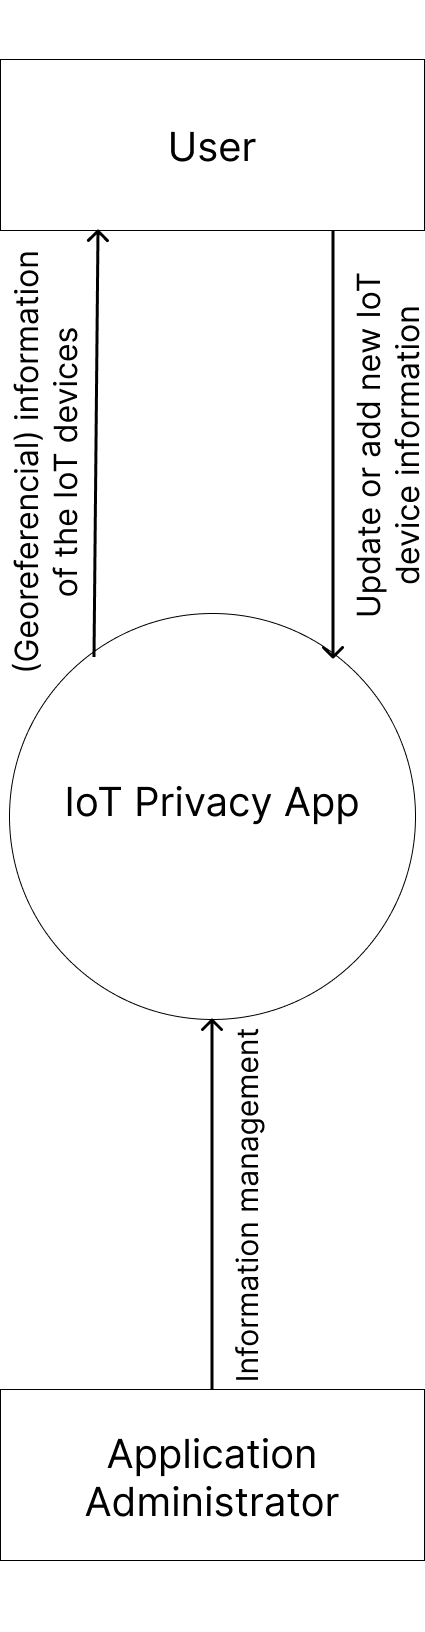
\includegraphics[width=3.5cm]{assets/images/contextual_diagram.png}
    \caption{IoT Privacy Contextual Diagram}
    \label{fig:contextual diagram}
\end{figure}
The contextual diagram is based on showing the actions performed with the
application. \\
\newline
User: \\
\newline
→ Receives:

- (Georeferencial) information of the IoT devices
\newline
→ Sends:

- Update or add new IoT device information \newline
\newline
Application Administrator (Programmer): \\
\newline
→ Receives:

- All information related to the application
\newline
→ Sends:

- Information management

\section{Data flow diagram}

A data flow diagram shows how information flows between the various entities
in the system and their relationships.
\begin{figure}[H]
    \centering
    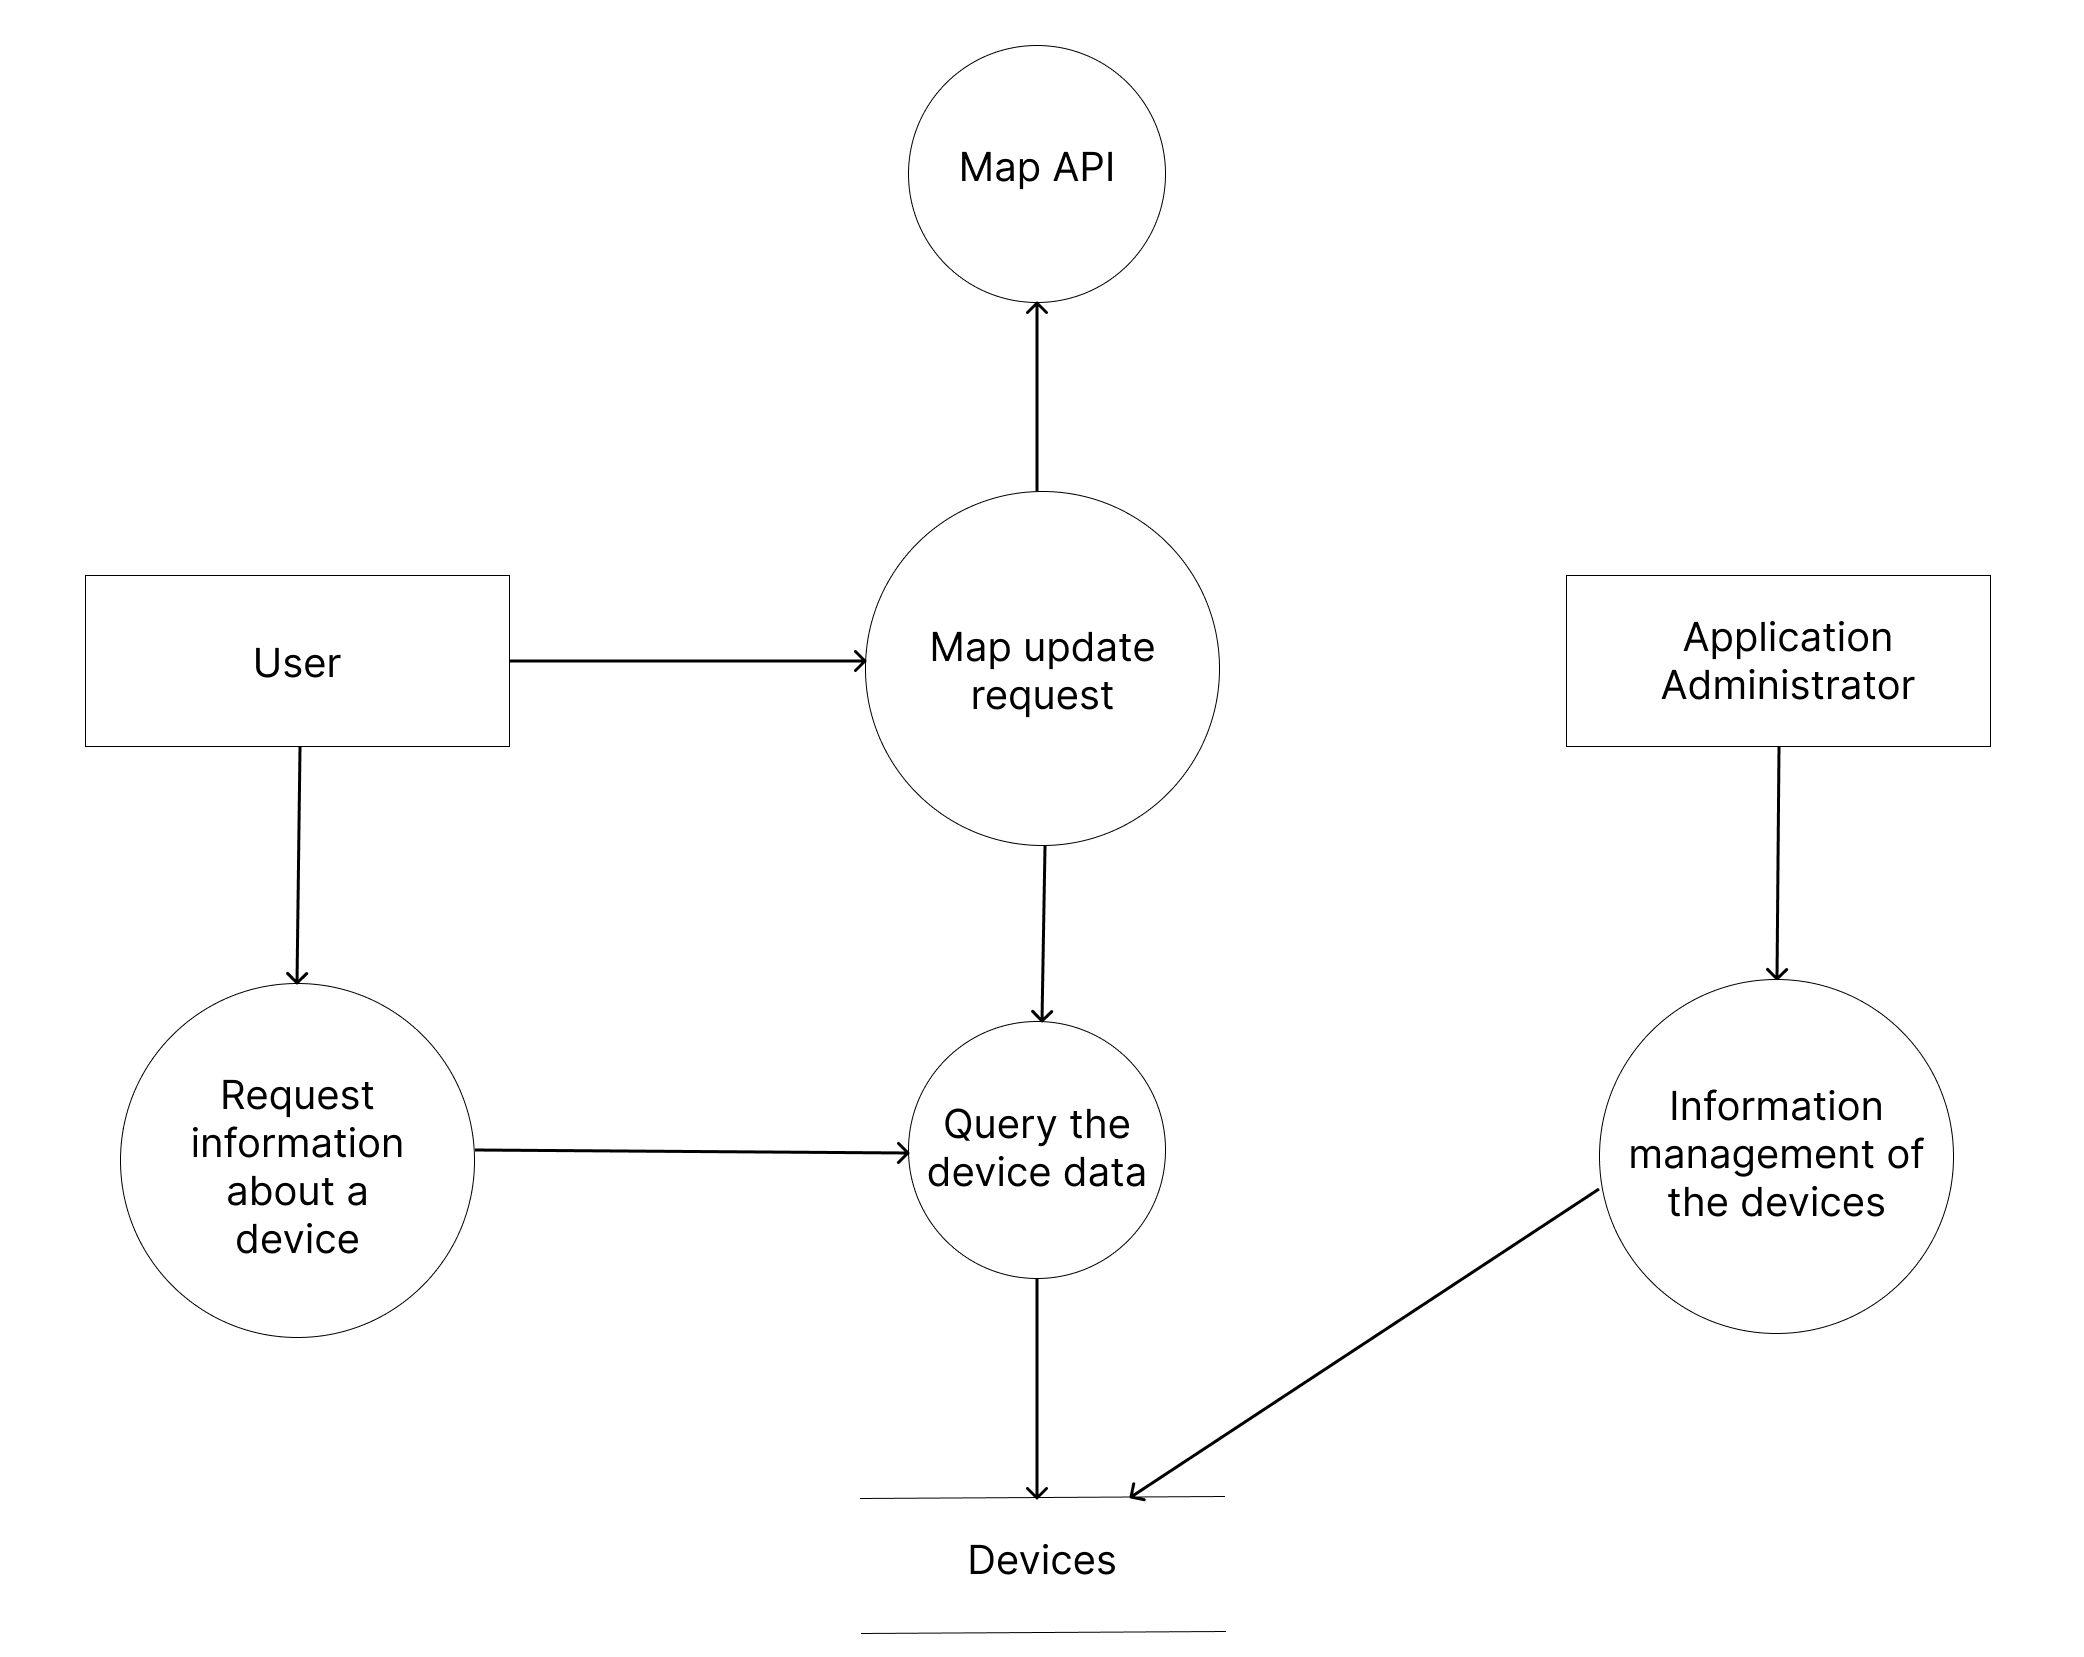
\includegraphics[width=15cm]{assets/images/data_flow_diagram.png}
    \caption{Data flow diagram}
    \label{fig:data flow diagram}
\end{figure}
The user can browse the application map, which will be created with an API,
and see the locations of the IoT devices, the user can also look up information
about the devices by clicking on a device on the map or by searching for
the device in the application. The administrator of the application is responsible for
its maintenance (correcting or deleting incorrect data), security and for
the veracity of the information.

\section{Swimlane diagram}

A swimlane diagram is a type of flowchart in which processes and decisions
are grouped into lanes. Parallel lines divide the diagram into lanes, each
lane being assigned to people/groups and application.
\begin{figure}[H]
    \centering
    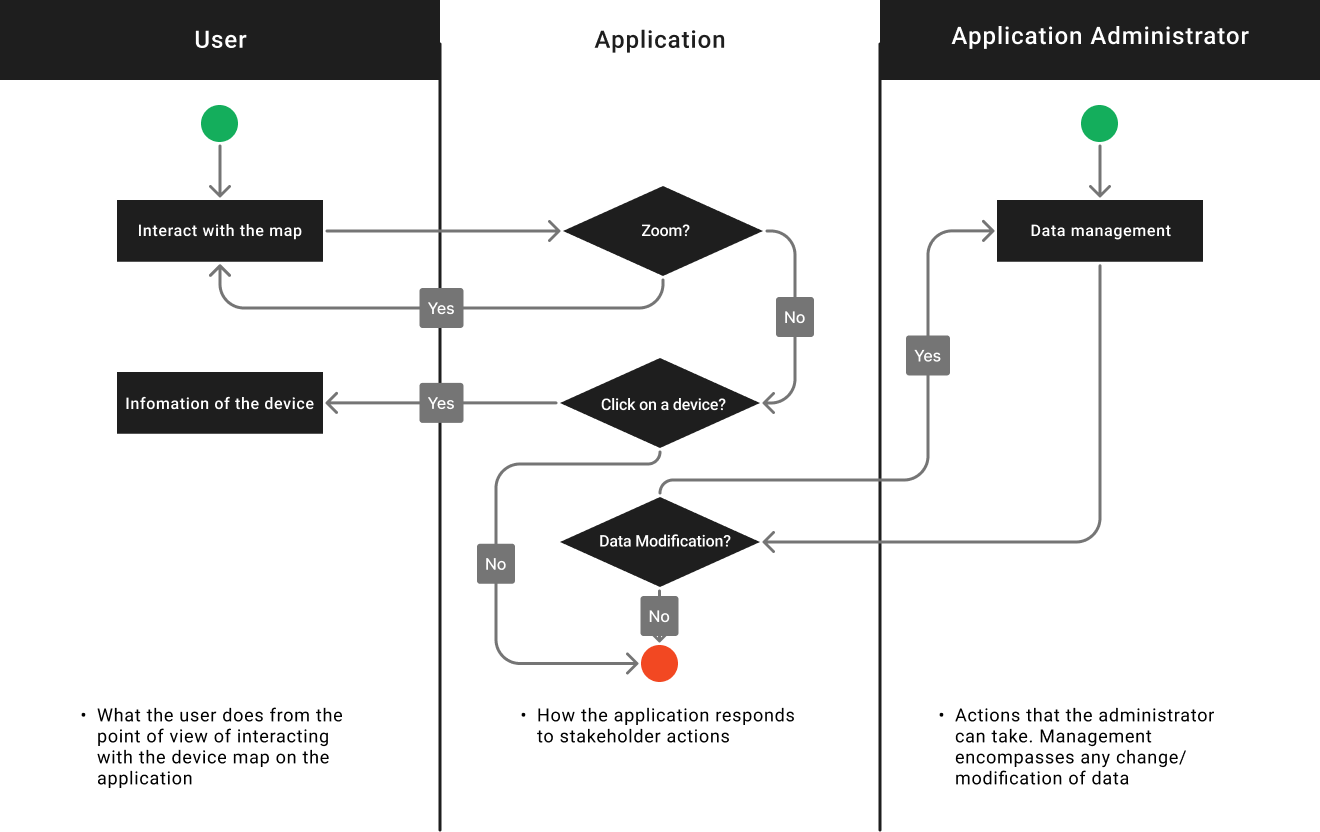
\includegraphics[width=15cm]{assets/images/swimlane_diagram.png}
    \caption{Swimlane diagram}
    \label{fig:diagram swimlane}
\end{figure}
This swimlane diagram represents a high level view of a possible user interaction
from the application's map, in this map the user can view the location of
IoT devices and can see more information about a particular device by selecting
it on the map. The application administrator, as mentioned above, can modify the
devices' data.

\chapter{System Features and Requirements}

\section{Business requirements}

Business requirements describe in business terms what must be delivered
or achieved to deliver value. It is what defines the way of doing business,
reflecting the internal policy, the defined process and/or the basic rules
of conduct.  In other words, it is a set of instructions that users already
follow and that the system to be developed must contemplate. Restrictions,
validations, conditions and process exceptions are classic examples of business
rules. A business rule will not necessarily be reflected in the system as
a functionality, but it will certainly determine the behaviour of one or
more functionalities of the system.
\newline
No business requirements have been identified for this project.

\section{Technology requirements}

Technology requirements describe what both hardware and software must be
used in order for a system to be realizable. In terms of hardware, it describes
what kind of physical components are needed for the software to work. The
software to be chosen must take into account the hardware that has been
chosen and what is intended by the stakeholders. This has implications for
how the system is implemented.
\newline
The technology requirements that have been identified for this project are as follows:
\begin{itemize}
    \item Firestore or similar database server
    \item Flutter framework with Dart being the main programming language
    \item Accessible on any smartphone (iOS or Android) \newline \textbf{Note}: No web based version it to be available.
\end{itemize}
These requirements have been chosen so that the system is available to as
many users as possible regardless of the hardware they use. The database
will allow to store the information that the users provide about the IoT
devices. The application will be developed with Flutter since it uses ahead
of time and just in time compilation with Dart as its programming language.
Flutter has better performance than React Native or a PWA stack and as such it is the chosen framework for
this application.

\section{Requirements table}

The requirements table identifies each feature and links each feature to an origin.
\newline
This is important to make it easier to manage requirements in the future.
Knowing the origin of the creation of the requirements makes it easier to
refer back to the source to clarify any questions.
\newline
A table was created with all the features found. For each feature it was identified
the users to which it is applied and the source.
\newline
For the features found were described the most appropriate requirements for
them. \\
\begin{table}[H]
    \centering
    \begin{adjustbox}{width=1.2\textwidth,center=\textwidth}
    % \rowcolors{5}{gray!10}{gray!40}
    \begin{tabular}{|l|p{0.2\textwidth}|p{0.2\textwidth}|p{0.4\textwidth}|p{0.15\textwidth}|}
        \hline
        \rowcolor{green!20}
        \textbf{R\#} & \textbf{Feature} & \textbf{Applicable stakeholders} & \textbf{Description} & \textbf{Source} \\
        \hline
        \textbf{1} & Navigate the map & User & \textbf{User}: The system should allow the user to scroll through the map of devices & \cite{nelson2023preparation} \\
        \hline
        \textbf{2} & Select device on the map & User & \textbf{User}: The system should allow the user to select a device on the map to view more information & \cite{nelson2023preparation} \\
        \hline
        \textbf{3} & Query devices through parameters & User & \textbf{User}: The system should allow the user to consult devices of only a certain type, data collected, general location & \cite{nelson2023preparation} \\
        \hline
        \textbf{4} & Query statistics of the devices & User & \textbf{User}: The system should allow consulting statistics of devices & \cite{nelson2023preparation} \\
        \hline
        \textbf{5} & Add a device & User & \textbf{User}: The system should allow the user to add a new device with name, category, data collected, location, etc. & \cite{nelson2023preparation} \\
        \hline
        \textbf{6} & Edit a device & User & \textbf{User}: The system should allow the user to change some data of a device & \cite{nelson2023preparation} \\
        \hline
        \textbf{7} & Delete a device & App Administrator & \textbf{App Administrator}: The system should allow the administrator to delete a device & \cite{nelson2023preparation} \\
        \hline
        \textbf{8} & Create account & User & \textbf{User}: The system shall allow a user to create an account. & \cite{nelson2023preparation} \\
        \hline
        \textbf{9} & Select privacy choices & User & \textbf{User}: The system shall allow the user to select their privacy choices for a certain device if the device allows for it. & \cite{nelson2023preparation} \\
        \hline
        \textbf{10} & See more information about privacy in IoT & User & \textbf{User}: The system shall allow the user to check what the terms used in the application mean. & Survey results \\
        \hline
    \end{tabular}
    \end{adjustbox}
    \caption{Requirements table}
    \label{table:table1}
\end{table}

\section{Functional requirements}

Functional requirements define the functions of a system or its components,
where functions are specifications or behaviours between system outputs and
inputs. \cite{fulton2017chapter} These describe what developers have to implement
so that users can complete tasks (user requirements), which in turn satisfy
business requirements. \cite{wiegers2013software} Functional requirements are
essential to the success of a project.
After building the tracing table the functional requirements that were needed
were extracted for each feature and grouped appropriately according to the
following groups:

\subsection{User Requirements}

\textbf{UR1} - The system shall allow the user to navigate through the devices georeferences;
\newline
\textbf{UR2} - The system shall allow the user to select a device on the map to view more information;
\newline
\textbf{UR4} - The system shall allow the user to consult devices of only a certain category, data collected, etc.;
\newline
\textbf{UR5} - The system shall allow consulting statistics of the devices;
\newline
\textbf{UR6} - The system shall allow the user to create an account;
\newline
\textbf{UR7} - The system shall allow a logged in user to add a new device with name, category, data collected, location, etc.;
\newline
\textbf{UR8} - The system shall allow a logged in user to change associated data of a device;

\subsection{Administrator Requirements}

\textbf{AR1} - The system shall allow a logged in administrator to add a new device with name, category, data collected, location, etc.;
\newline
\textbf{AR2} - The system shall allow a logged in administrator to change associated data of a device;
\newline
\textbf{AR3} - The system shall allow a logged in administrator to delete a device;

\subsection{System requirements}

\textbf{SR1} - The system shall generate statistics related to the IoT devices that reside in the database;

\section{Non-functional requirements}

\textbf{NFR1} - The system shall behave the same in different platforms (Android and iOS);

\chapter{Use cases}

\section{Use cases diagram}

The use cases diagram provides a high level visualisation of the user
requirements. The box represents the system boundary. An actor's arrow
for a use case indicates that he is the primary actor for it.
The primary actor initiates the use case and derives the primary value
from it. \cite{wiegers2013software}
\begin{figure}[H]
    \centering
    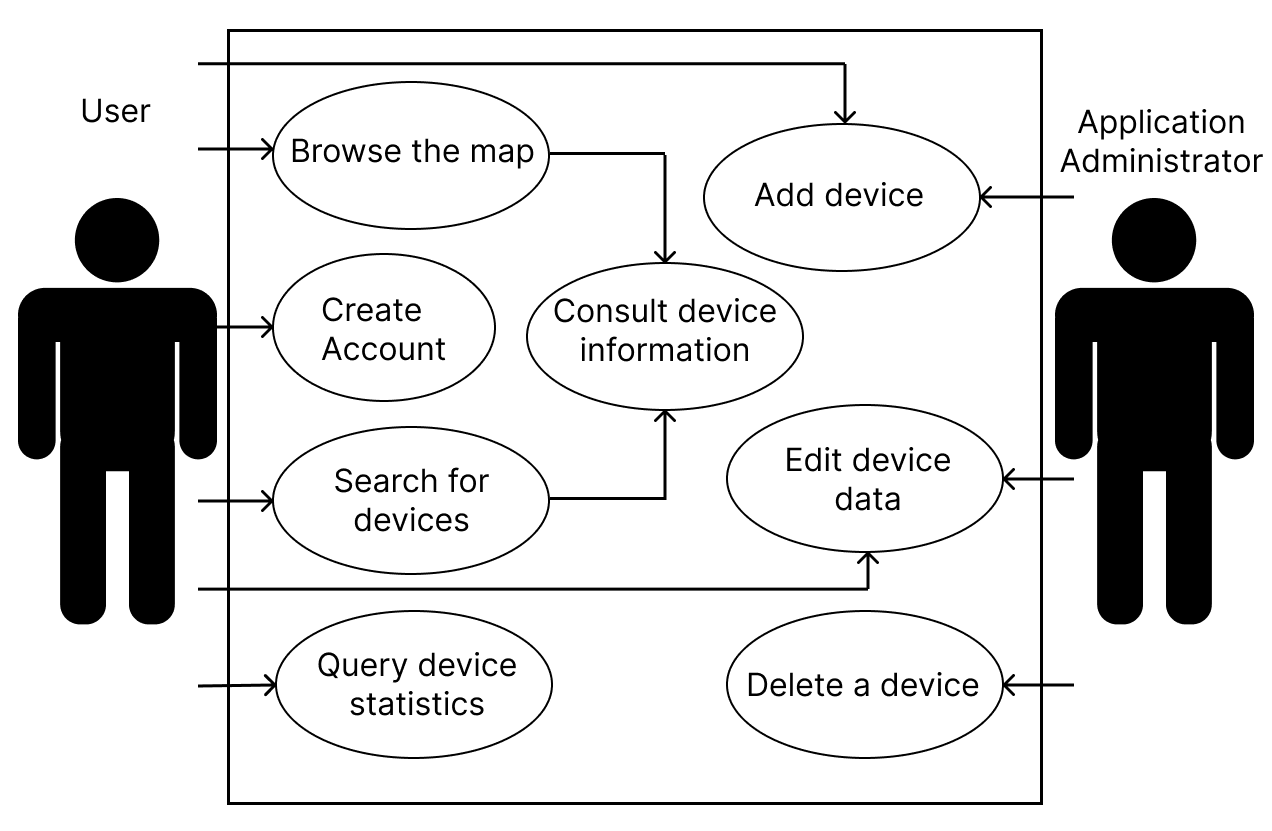
\includegraphics[width=15cm]{assets/images/use_cases_diagram.png}
    \caption{Use cases diagram}
    \label{fig:use cases diagram}
\end{figure}

\section{Use cases}

A use case is a type of classifier representing a
coherent functional unit provided by the system, subsystem, or class manifested
by sequences of interchangeable messages between systems and one or more
actors. \cite{UseUsability}
\newline
This technique describes the tasks that users need to perform with
the system or the user-system interaction that may be important to some
stakeholders. They also help in testing by checking that the functionality
has been implemented correctly. The use cases uses an Unified Modeling
Language (UML) notation.

\begin{table}[H]
    \centering
    \begin{adjustbox}{width=1.2\textwidth,center=\textwidth}
        \begin{tabular}{|m{4cm}|m{12cm}|}
            \hline
            ID and Name: & UC-01 Query devices through certain parameters \\
            \hline
            Created By: & Nelson Vieira 20/02/2023 \\
            \hline
            Primary Actor: & End User \\
            \hline
            Description: & The user makes a device information query \\
            \hline
            Trigger: & The user wants to search device information \\
            \hline
            Pre-conditions: & N/A \\
            \hline
            Post-conditions: & POST-1. The user finds device information \\
            \hline
            Normal Flow: & \textbf{1.0 Query information of a device on the map}
            \begin{enumerate}
                \item The user browses the map
                \item The user clicks on the icon to show some information about the device
                \item The user clicks on the device pop-up
            \end{enumerate} \\
            \hline
            Alternative Flow: & \textbf{1.1 Device information search}
            \begin{enumerate}
                \item User enters device name
                \item The user chooses the device he wants from a list generated from the search performed
            \end{enumerate} \\
            \hline
            Alternative Flow: & \textbf{1.2 Alternative search for information from a device}
            \begin{enumerate}
                \item The user selects one of the parameters:
                \begin{enumerate}
                    \item Category
                    \item Name
                \end{enumerate}
                \item The user chooses the device he wants from a list generated from the search carried out
            \end{enumerate} \\
            \hline
            Exceptions: & \textbf{1.0.E1  The API is not working}
            \begin{enumerate}
                \item The system displays an alert message: ``We are having connection problems, please wait for a while''
            \end{enumerate} \\
            \hline
            Priority: & High \\
            \hline
            Business Requirements: & N/A \\
            \hline
            Assumptions: & N/A \\
            \hline
        \end{tabular}
    \end{adjustbox}
    \caption{Use case 1 - device information query}
    \label{use case 1}
\end{table}

\begin{table}[H]
    \centering
    \begin{adjustbox}{width=1.2\textwidth,center=\textwidth}
        \begin{tabular}{|m{4cm}|m{12cm}|}
            \hline
            ID and Name: & UC-02 Device statistics query \\
            \hline
            Created By: & Nelson Vieira 20/02/2023 \\
            \hline
            Primary Actor: & End User \\
            \hline
            Description: & The user queries the statistics of the devices \\
            \hline
            Trigger: & The user wants to find statistics of devices \\
            \hline
            Pre-conditions: & N/A \\
            \hline
            Post-conditions: & POST-1. The system displays the statistics of the devices \\
            \hline
            Normal Flow: & \textbf{2.0 Device statistics query}
            \begin{enumerate}
                \item User selects statistics tab
                \item The user can only select certain parameters, such as:
                \begin{enumerate}
                    \item Category
                    \item Location
                \end{enumerate}
            \end{enumerate} \\
            \hline
            Alternative Flow: & N/A \\
            \hline
            Exceptions: & \textbf{2.0.E1  The API is not working}
            \begin{enumerate}
                \item The system displays an alert message: ``We are having connection problems, please wait for a while''
            \end{enumerate} \\
            \hline
            Priority: & Medium \\
            \hline
            Business Requirements: & N/A \\
            \hline
            Assumptions: & N/A \\
            \hline
        \end{tabular}
    \end{adjustbox}
    \caption{Use case 2 - statistics query}
    \label{use case 2}
\end{table}

\begin{table}[H]
    \centering
    \begin{adjustbox}{width=1.15\textwidth,center=\textwidth}
        \begin{tabular}{|m{4cm}|m{12cm}|}
            \hline
            ID and Name: & UC-03 Add a device \\
            \hline
            Created By: & Nelson Vieira 22/02/2023 \\
            \hline
            Primary Actor: & End User \\
            \hline
            Description: & Addition of a new IoT device in the application \\
            \hline
            Trigger: & The user wants to add a new IoT device \\
            \hline
            Pre-conditions: & N/A \\
            \hline
            Post-conditions: & POST-1. A new IoT device is added to the application \\
            \hline
            Normal Flow: & \textbf{3.0 Add a device}
            \begin{enumerate}
                \item The user enters the following data of a new IoT device:
                \begin{enumerate}
                    \item Name
                    \item Type of data collected
                    \item Category
                    \item Photos
                \end{enumerate}
                \item The user clicks submit
                \item The user adds the location of the IoT device on the map
            \end{enumerate} \\
            \hline
            Alternative Flow: & N/A \\
            \hline
            Exceptions: & \textbf{3.0.E1  The device is already in the database}
            \begin{enumerate}
                \item The system displays an error message
            \end{enumerate} \\
            \hline
            Priority: & High \\
            \hline
            Business Requirements: & N/A \\
            \hline
            Assumptions: & N/A \\
            \hline
        \end{tabular}
    \end{adjustbox}
    \caption{Use case 3 - add a device}
    \label{use case 3}
\end{table}

\begin{table}[H]
    \centering
    \begin{adjustbox}{width=1.1\textwidth,center=\textwidth}
        \begin{tabular}{|m{4cm}|m{12cm}|}
            \hline
            ID and Name: & UC-04 Edit a device's data \\
            \hline
            Created By: & Nelson Vieira 22/02/2023 \\
            \hline
            Primary Actor: & End User \\
            \hline
            Description: & Editing the data of an IoT device in the application \\
            \hline
            Trigger: & The user wants to edit an IoT device's data \\
            \hline
            Pre-conditions: & N/A \\
            \hline
            Post-conditions: & POST-1. The data that has been changed appears in the application \\
            \hline
            Normal Flow: & \textbf{4.0 Edit a device's data}
            \begin{enumerate}
                \item The user can change any of the following device data:
                \begin{enumerate}
                    \item Name
                    \item Category
                    \item Photos
                \end{enumerate}
                \item The user clicks on submit
            \end{enumerate} \\
            \hline
            Alternative Flow: & N/A \\
            \hline
            Exceptions: &
            % Exceptions: & \textbf{4.0.E1  Unique data already registered}
            % \begin{enumerate}
            %     \item The system displays an error message
            %     \item The system asks the user to enter different data
            % \end{enumerate}
            \textbf{4.0.E1  The device to be edited has been deleted in the meantime}
            \begin{enumerate}
                \item The system displays an error message
                \item The system prohibits editing
            \end{enumerate} \\
            \hline
            Priority: & High \\
            \hline
            Business Requirements: & N/A \\
            \hline
            Assumptions: & N/A \\
            \hline
        \end{tabular}
    \end{adjustbox}
    \caption{Use case 4 - edit a device's data}
    \label{use case 4}
\end{table}

\begin{table}[H]
    \centering
    \begin{adjustbox}{width=1.2\textwidth,center=\textwidth}
        \begin{tabular}{|m{4cm}|m{12cm}|}
            \hline
            ID and Name: & UC-05 Delete a device \\
            \hline
            Created By: & Nelson Vieira 22/02/2023 \\
            \hline
            Primary Actor: & App Administrator \\
            \hline
            Description: & Deleting a device in the application \\
            \hline
            Trigger: & The administrator wants to delete a device \\
            \hline
            Pre-conditions: & PRE-1. The device to be deleted must be in the application's database \\
            \hline
            Post-conditions: & POST-1. The device is deleted from the application \\
            \hline
            Normal Flow: & \textbf{5.0 Delete a device}
            \begin{enumerate}
                \item The administrator deletes a device, through:
                \begin{enumerate}
                    \item ID of device
                    \item Name of device
                \end{enumerate}
                \item The administrator confirms the deletion
                \item The system deletes the device
            \end{enumerate} \\
            \hline
            Alternative Flow: & N/A \\
            \hline
            Exceptions: & \textbf{5.0.E1  The device to be deleted no longer exists in the database}
            \begin{enumerate}
                \item The system displays an error message
                \item The system prohibits deletion
            \end{enumerate} \\
            \hline
            Priority: & High \\
            \hline
            Business Requirements: & N/A \\
            \hline
            Assumptions: & It is assumed that the administrator has database access \\
            \hline
        \end{tabular}
    \end{adjustbox}
    \caption{Use case 5 - delete a device}
    \label{use case 5}
\end{table}

\begin{table}[H]
    \centering
    \begin{adjustbox}{width=1.2\textwidth,center=\textwidth}
        \begin{tabular}{|m{4cm}|m{12cm}|}
            \hline
            ID and Name: & UC-06 Create an account \\
            \hline
            Created By: & Nelson Vieira 22/02/2023 \\
            \hline
            Primary Actor: & End User \\
            \hline
            Description: & Create a new end user account \\
            \hline
            Trigger: & The user wants to create an account \\
            \hline
            Pre-conditions: & PRE-1. The user wants to add a new device \\
            \hline
            Post-conditions: & POST-1. The account is created in the application \\
            \hline
            Normal Flow: & \textbf{6.0 Account creation process}
            \begin{enumerate}
                \item The user enter the following data in the register screen:
                \begin{enumerate}
                    \item Username
                    \item Email
                    \item Password
                \end{enumerate}
                \item The system adds the account data to the database
                \item An account confirmation email is sent to the email provided by the user
                \item The user confirms the account
            \end{enumerate} \\
            \hline
            Alternative Flow: & N/A \\
            \hline
            Exceptions: & \textbf{6.0.E1  The username already exists in the database}
            \begin{enumerate}
                \item The system displays an error message
                \item The system allows the user to recover the account
            \end{enumerate}
            \textbf{6.0.E2 The email already exists in the database}
            \begin{enumerate}
                \item The system displays an error message
                \item The system allows the user to recover the account
            \end{enumerate} \\
            \hline
            Priority: & High \\
            \hline
            Business Requirements: & N/A \\
            \hline
            Assumptions: & N/A \\
            \hline
        \end{tabular}
    \end{adjustbox}
    \caption{Use case 6 - create an account}
    \label{use case 6}
\end{table}

\chapter{Requirements prioritisation}

Regarding the prioritization of requirements, the Quality Function Deployment technique
proposed by Cohen in 1995 \cite{cohen1995quality} is used to estimate the priority of a group of requirements.
This is based on the benefit of including a feature/requirement, the penalty of not including
it, and also the cost and risks associated with implementation. With the MoSCoW method \cite{clegg1994case}, the
initial features are reduced to facilitate the use of the Quality Function Deployment table.
\newline
In this approach the values 0 and 1 are used. In case of 1 it means that the column requirement/feature
is a higher priority than the row one and if it is 0 the opposite is true.

\begin{table}[H]
    \centering
    % \rowcolors{5}{gray!10}{gray!40}
    \begin{tabular}{|>{\columncolor{gray!10!white}}r|r|r|r|r|r|r|r|r|r|r|}
        \hline
        \rowcolor{gray!10!white}
        & R\#1 & R\#2 & R\#3 & R\#4 & R\#5 & R\#6 & R\#7 & R\#8 & R\#9 & R\#10 \\
        \hline
        R\#1 && 0 & 0 & 0 & 1 & 0 & 0 & 0 & 0 & 0 \\
        \hline
        R\#2 & 1 && 0 & 0 & 1 & 0 & 0 & 0 & 0 & 0 \\
        \hline
        R\#3 & 1 & 1 && 0 & 1 & 0 & 0 & 0 & 0 & 0 \\
        \hline
        R\#4 & 1 & 1 & 1 && 1 & 0 & 0 & 0 & 1 & 1 \\
        \hline
        R\#5 & 0 & 0 & 0 & 0 && 0 & 0 & 1 & 1 & 1 \\
        \hline
        R\#6 & 1 & 1 & 1 & 1 & 1 && 0 & 0 & 1 & 1 \\
        \hline
        R\#7 & 1 & 1 & 1 & 1 & 1 & 1 && 1 & 1 & 1 \\
        \hline
        R\#8 & 1 & 1 & 1 & 1 & 0 & 1 & 0 && 1 & 1 \\
        \hline
        R\#9 & 1 & 1 & 1 & 0 & 0 & 0 & 0 & 0 && 1 \\
        \hline
        R\#10 & 1 & 1 & 1 & 0 & 0 & 0 & 0 & 0 & 0 & \\
        \hline
        \rowcolor{gray!50}
        Total & 8 & 7 & 6 & 3 & 6 & 2 & 0 & 2 & 5 & 6 \\
        \hline
    \end{tabular}
    \caption{Prioritisation table using the MoSCoW technique}
    \label{table:tabela moscow}
\end{table}

After this initial selection, a prioritisation table is created where it is measured, on a scale of
1 to 9, to rank the benefit and penalty of each requirement. The cost and implementation risk
associated to each feature is also estimated.

\begin{table}[H]
    \centering
    \begin{adjustbox}{width=1.2\textwidth,center=\textwidth}
    \begin{tabular}{|>{\columncolor{gray!10!white}}r|r|r|r|r|r|r|r|r|r|r|}
        \hline
        \rowcolor{gray!10!white}
        \multicolumn{2}{|c|}{\textbf{Feature}} & \textbf{Relative benefit} & \textbf{Relative penalty} & \textbf{Total value} & \textbf{Value \%} & \textbf{Relative cost} & \textbf{Cost \%} & \textbf{Relative risk} & \textbf{Risk \%} & \textbf{Priority} \\
        \hline
        Navigate the map & 1 & 9 & 9 & 27 & 13,24 & 5 & 10,42 & 5 & 10,00 & 0,65 \\
        \hline
        Select device on the map & 2 & 9 & 9 & 27 & 13,24 & 5 & 10,42 & 5 & 10,00 & 0,65 \\
        \hline
        Add a device & 5 & 9 & 9 & 27 & 13,24 & 3 & 6,25 & 4 & 8,00 & 0,93 \\
        \hline
        See more information about privacy in IoT & 10 & 5 & 6 & 24 & 11,76 & 6 & 12,50 & 2 & 4,00 & 0,71 \\
        \hline
        Query devices through parameters & 3 & 6 & 8 & 20 & 9,80 & 7 & 14,58 & 6 & 12,00 & 0,37 \\
        \hline
        Select privacy choices & 9 & 5 & 7 & 19 & 9,31 & 6 & 12,50 & 8 & 16,00 & 0,33 \\
        \hline
        Query statistics of the devices & 4 & 3 & 5 & 11 & 5,39 & 5 & 10,42 & 7 & 14,00 & 0,22 \\
        \hline
        Create account & 8 & 8 & 9 & 15 & 7,35 & 5 & 10,42 & 5 & 10,00 & 0,36 \\
        \hline
        Edit a device & 6 & 7 & 8 & 22 & 10,78 & 3 & 6,25 & 4 & 8,00 & 0,76 \\
        \hline
        Delete a device & 7 & 4 & 4 & 12 & 5,88 & 3 & 6,25 & 4 & 8,00 & 0,41 \\
        \hline
        \rowcolor{gray!50}
        \multicolumn{2}{|c|}{\textbf{Total}} & 67 & 62 & \textbf{198} & 100,00 & \textbf{39} & 100,00 & \textbf{37} & 100,00 & \\
        \hline
    \end{tabular}
    \end{adjustbox}
    \caption{Features prioritisation table}
    \label{table:tabela de priorizacao}
\end{table}

Using this method we get the requirements sorted by priority:

\begin{table}[H]
    \centering
    % \rowcolors{5}{gray!10}{gray!40}
    \begin{tabular}{|c|c|c|c|}
        \hline
        \rowcolor{gray!50}
        \textbf{Rank} & \textbf{Feature} & \textbf{\# Feature} & \textbf{Priority} \\
        \hline
        1 & Add a device & 5 & 0,93 \\
        \hline
        2 & Edit a device & 6 & 0,76 \\
        \hline
        3 & See more information about privacy in IoT & 10 & 0,71 \\
        \hline
        4 & Navigate the map & 1 & 0,65 \\
        \hline
        5 & Select device on the map & 2 & 0,65 \\
        \hline
        6 & Delete a device & 7 & 0,41 \\
        \hline
        7 & Query devices through parameters & 3 & 0,37 \\
        \hline
        8 & Create an account & 8 & 0,36 \\
        \hline
        9 & Select privacy choices & 9 & 0,33 \\
        \hline
        10 & Query statistics of the devices & 4 & 0,22 \\
        \hline
    \end{tabular}
    \caption{Highest priority requirements ordered}
    \label{table:sorted requirements}
\end{table}

\section{Acceptance Criteria}

To make it easier to test whether the highest priority features that were chosen
previously were well implemented, these acceptance criteria were created for each
of them. These criteria help us understand the minimum conditions for this
application to be considered an MVP, i.e., for this project to have the minimum
possible requirements in order for it to be considered production ready.
\newline
For these acceptance criteria the following was considered:

\begin{itemize}
    \item High-level functionality that must be present for the system to be usable
    \item Non-functional criteria and quality metrics that have to be satisfied
    \item Possibility of open problems or defects (we can guarantee that no defects or TBD is present for the system to be accepted)
    \item Legal or contractual restrictions (that have to be met for the system to be accepted)
\end{itemize}

\subsection{Features}

\subsubsection{Add a device}

\begin{itemize}
    \item The system allows the user to add a new device that is not yet present in the database
\end{itemize}

\subsubsection{Edit a device}

\begin{itemize}
    \item The system allows the editing of an existing device
    \item The system saves in the database the changes that have been made
\end{itemize}

\subsubsection{Delete a device}

\begin{itemize}
    \item The system allows the deletion of an existing device
    \item The system deletes the device from its database
\end{itemize}

\subsubsection{Navigate the map}

\begin{itemize}
    \item The system can represent the devices on the map
    \item The system allows the user to navigate throughout the map and view the devices
\end{itemize}

\subsubsection{Query devices through parameters}

\begin{itemize}
    \item The system allows searching devices by the certain parameters like the category, the type of data collected
\end{itemize}

\subsubsection{Select device on map}

\begin{itemize}
    \item The system allows the user to select a device on the map
\end{itemize}

\subsubsection{See more information about privacy in IoT}

\begin{itemize}
    \item The system allows the user to see more information about privacy in IoT
\end{itemize}

\subsubsection{Select privacy choices}

\begin{itemize}
    \item The system allows the user to select a device and view its details
    \item The system allows the user to select privacy choices for that device (if that option is available)
\end{itemize}

\subsubsection{Consult devices' statistics}

\begin{itemize}
    \item The system allows the user to consult statistics concerning the devices
\end{itemize}

\subsubsection{Create account}

\begin{itemize}
    \item The system allows the creation of an account
    \item The user has to enter its username, email and a password
    \item The system can detect whether the email is already in use
    \item The system can send a profile creation confirmation email
    \item The user can confirm the profile creation
    \item The system allows the user to sign in
\end{itemize}

\section{Prototype}

For the prototype several drafts are first made with design tools, such as Figma or . Then,
with the tools previously mentioned in \textbf{Technology Requirements}, an application is created.

\bibliographystyle{IEEEtran}
\bibliography{assets/references}

\end{document}
